\chapter{Modeling}
The objective of this thesis is the grouping of expenses with the methods of \ac{NLP}. Grouping, or clustering, is the practise of sorting data points into groups in such a way that the similarity inside a group (intra-cluster similarity) is high while the similarity between clusters (inter-cluster similarity) is low. The defintion of similarity as well as different clustering algorithms are presented and contrasted in the following sections.


\section{Alternatives}
\subsection{Similarity and distance measures}
A distance measure is a quantification of how near objects in space are. Distance measures can be defined for spaces of arbitrary numbers of dimensions. In the examples, four words (man, woman, king, queen) are compared in their semantic similarity. The word vectors were generated with a word embedding, but the focus is on comparing the distance measures available for clustering later on.

		\begin{figure}[!h]
			\centering
			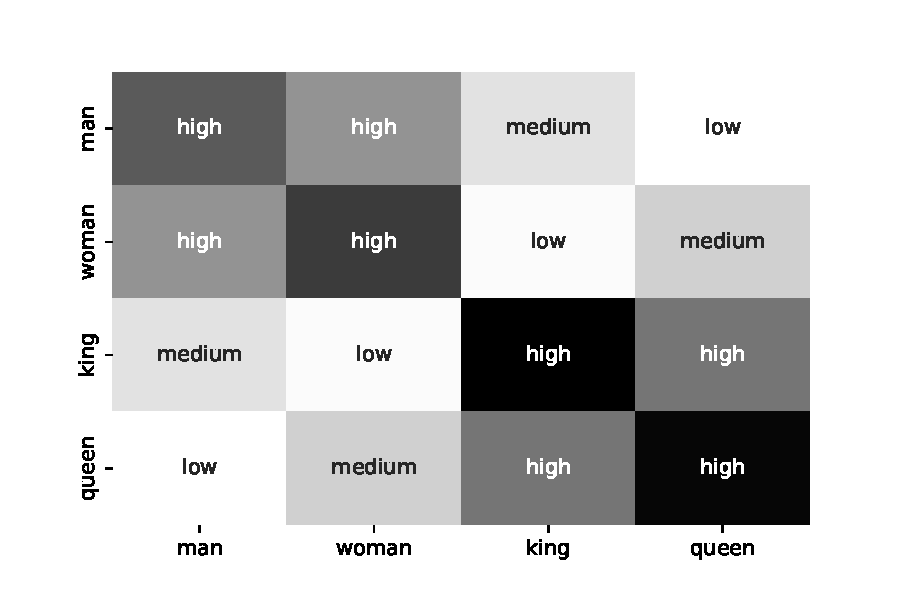
\includegraphics[height=6cm]{Bilder/models/heatmap_dot_product.pdf}
			\caption{Dot Product as Similarity Measure}
			\label{fig:dotproduct-heatmap}
		\end{figure}
	
		\subparagraph{Dot Product}
		The dot product is an operation transforming a vector into a scalar through multiplying the vectors element-wise. This operation is easily and efficiently calculated, but has some pitfalls.
		While every word in the example (\ref{fig:dotproduct-heatmap}) ranks very high in similarity to itself, the distance between the word and itself is not always the same for every word. This happens because the dot product is not agnostic of a vector's magnitude. A vector's product with itself is the square of its magnitude. This results in the similarity of man-man to be lower than the similarity of queen-queen.
		This fact makes the dot product impractical for accurately representing the relationships of words.
	
					\[ 
				\text{dot product} :=  \mathbf{A} \cdot \mathbf{B}= \sum\limits_{i=1}^{n}{A_i  B_i} 
				\]

	
		\subparagraph{Euclidean Distance} \label{euclidean}
		For low-dimensional applications, this distance works well and shows great results. Euclidean distance can be calculated in a highly efficient manner, even for n dimensions. This suggests, that euclidean distance is particularly suitable for high-dimensional data. Unfortunately, euclidean distance falls victim to the curse of dimensionality. In \cite[p.~1]{beyerNearestNeighbor} it is proven that with increasing dimensions, the distance between data points approaches an uniform value for all data points. This effect could be demonstrated for spaces with as little as ten dimensions. Therefore, it can be said that euclidean distance is not suitable for high-dimensional data. With vectors in \ac{NLP} ranging from 100 to 800 dimensions with embeddings and hundreds of thousands with \ac{TF-IDF}, this distance measure is not suitable.
		
				\[ 
		\text{euclidean distance} :=  \sum\limits_{i=1}^{n}{(A_i -  B_i)^{2}} 
		\]
		
		\begin{figure} 
			\begin{minipage}{0.49\textwidth}
				\label{fig:euclidean}
				
				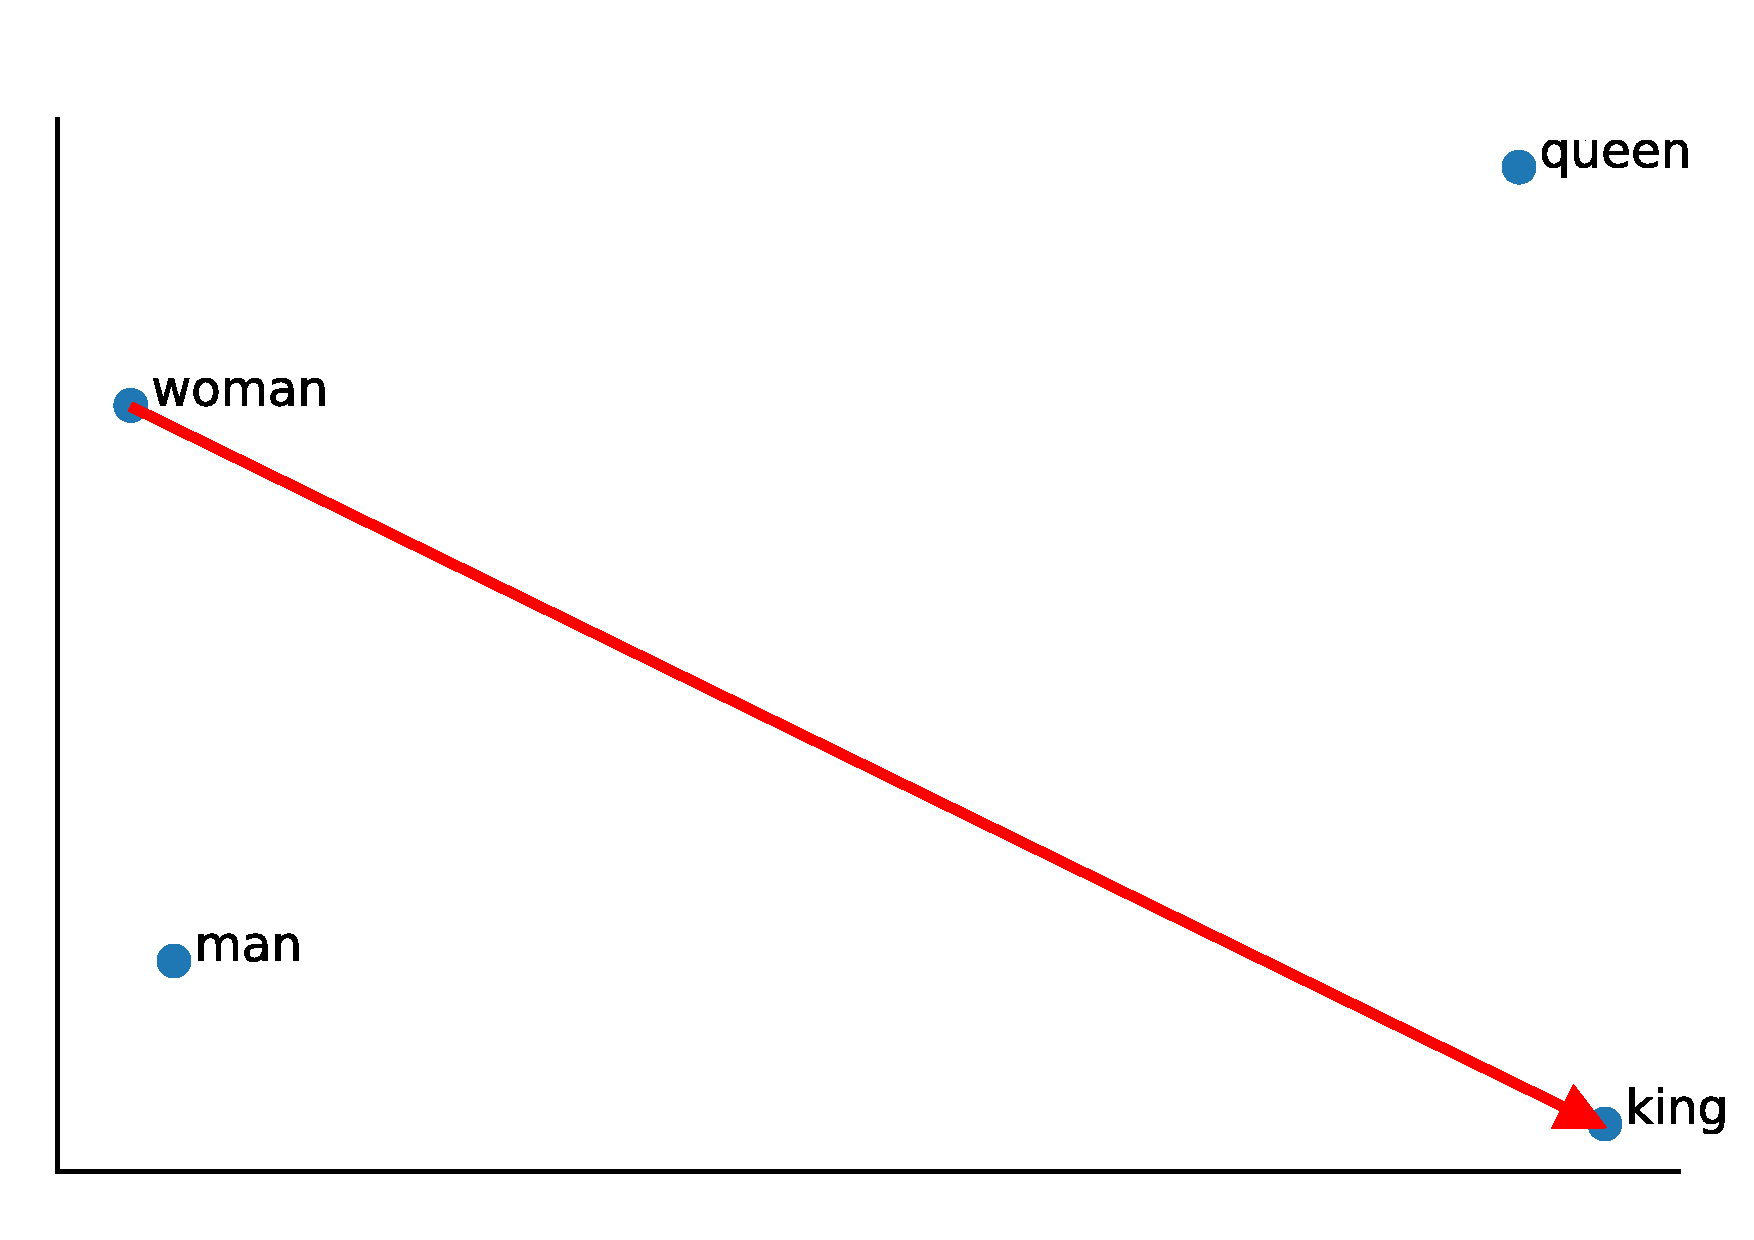
\includegraphics[height=5cm]{Bilder/models/euclidean}
				\caption{Euclidean Distance as Measure}
			\end{minipage}
			\hfill
			\begin{minipage}{0.49\textwidth}
				\label{fig:cosine}
				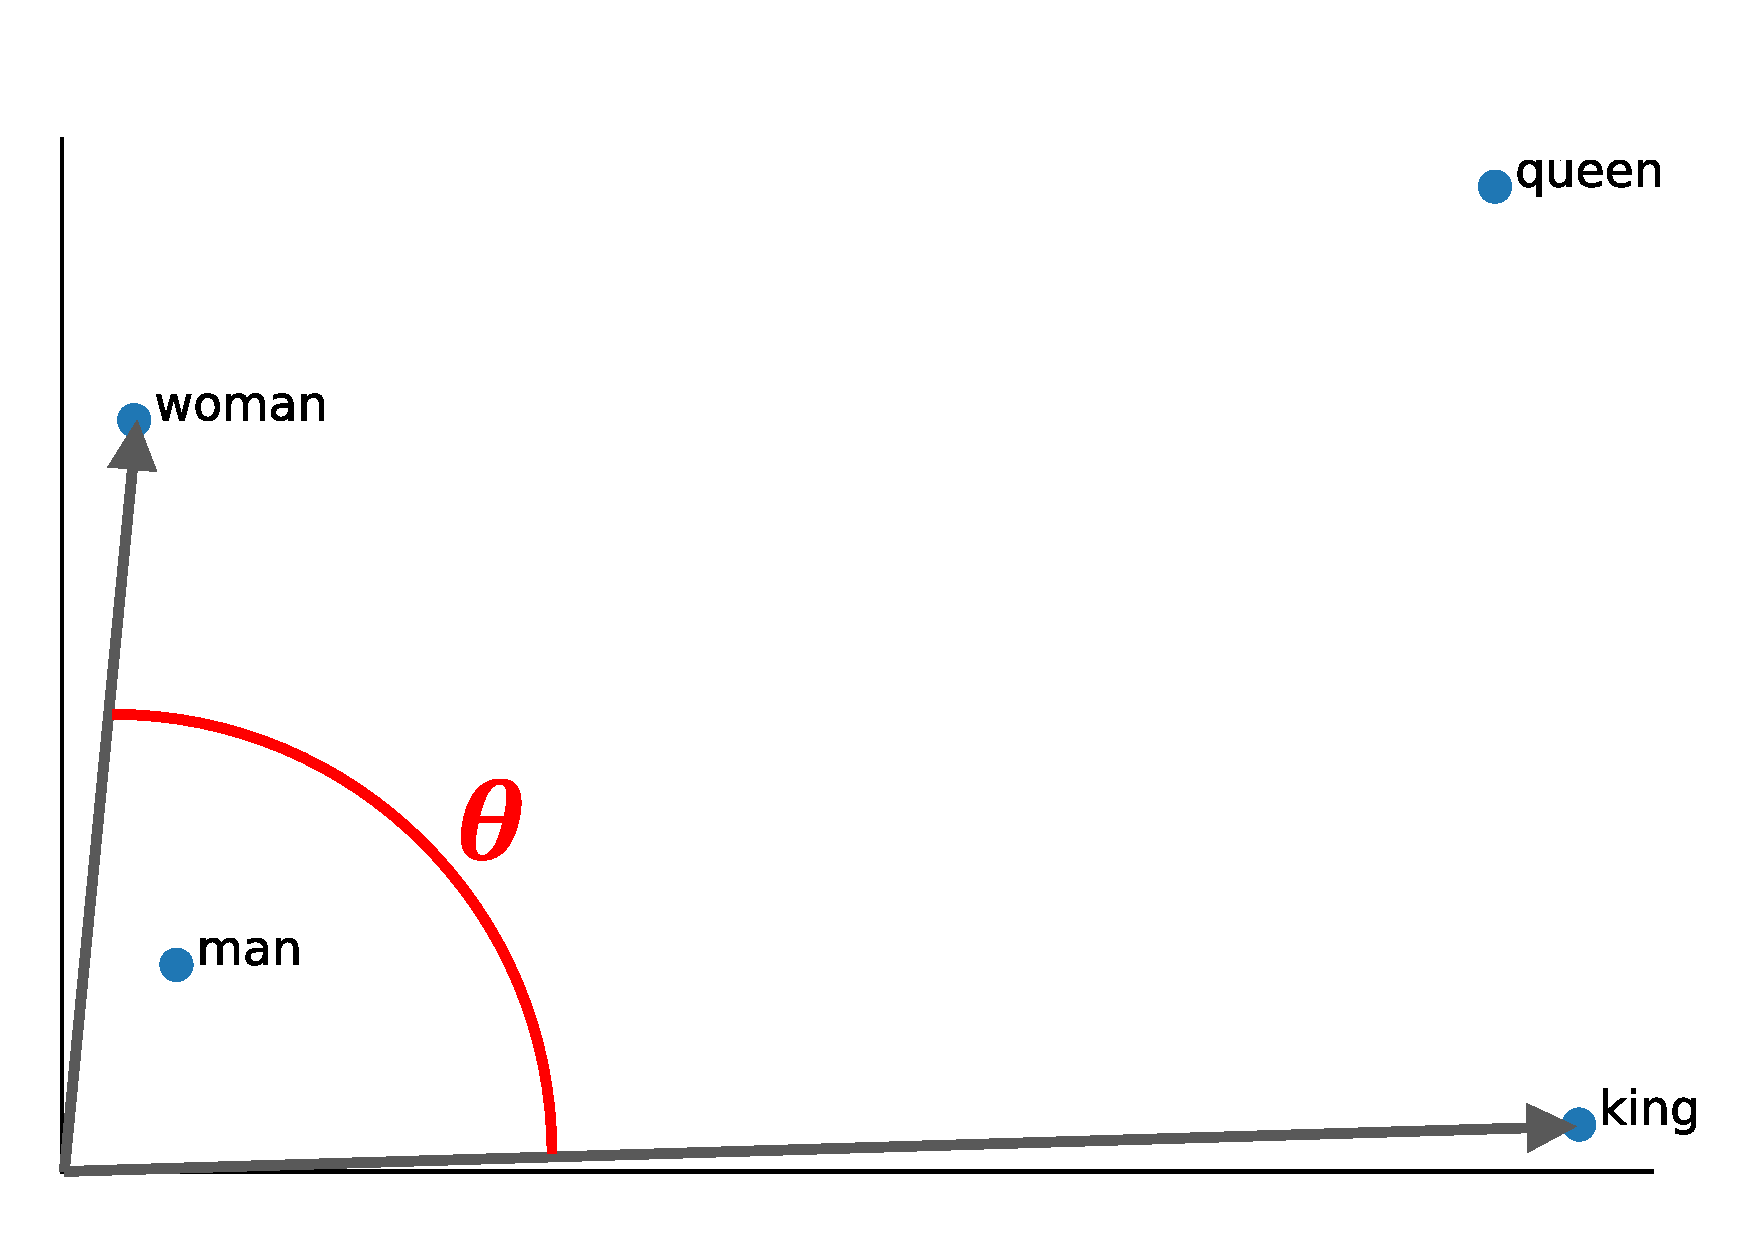
\includegraphics[height=5cm]{Bilder/models/cosine}
				\caption{Cosine Similarity as Measure}
			\end{minipage}
			\hfill
		\end{figure} 
	
		\subparagraph{Cosine Similarity}
		The name of this measure already suggests that not distance but similarity of objects is measured. Instead, it quantifies how close two vectors are. The euclidean distance does not perform well in high-dimensional space, but cosine similarity is highly accurate even for high-dimensional data  \cite{40algorithms}. Mathematically, the cosine distance is the cosine of the angle between two vectors. A wide angle means a high distance between two vectors, or in this case two words. Narrow angles stand for a low distance and words being closely related. In example \ref{fig:cosine}, the word vectors for woman and king have a higher angle than those of woman and queen. This means the words woman and queen are more similar thank woman and king.
		
		\[ 
		\text{cosine similarity} := \cos(\theta) = {\mathbf{A} \cdot \mathbf{B} \over \|\mathbf{A}\| \|\mathbf{B}\|} = \frac{ \sum\limits_{i=1}^{n}{A_i  B_i} }{ \sqrt{\sum\limits_{i=1}^{n}{A_i^2}}  \sqrt{\sum\limits_{i=1}^{n}{B_i^2}} }
		  \]
		
		
\subsection{Clustering Algorithms}
		
		\subparagraph{K-Means}
		The k-Means algorithm generates $k$ groups of data by iteratively adapting clusters and their centers. The algorithm is mainly focused on performance, hence the design is kept lean by omitting logic for determining the number of clusters \cite[c.~6.2]{40algorithms}. Following pseudo code illustrates the workings of the algorithm.
		
		\begin{lstlisting}
randomly choose k_centers
while (iterations < max_iterations):
	assign each point to nearest center in k_centers
	mean of each cluster's elements are k_centers_new
	if k_centers == k_centers_new:
		break
		\end{lstlisting}
	
			 \begin{figure}[!h]
		\centering
		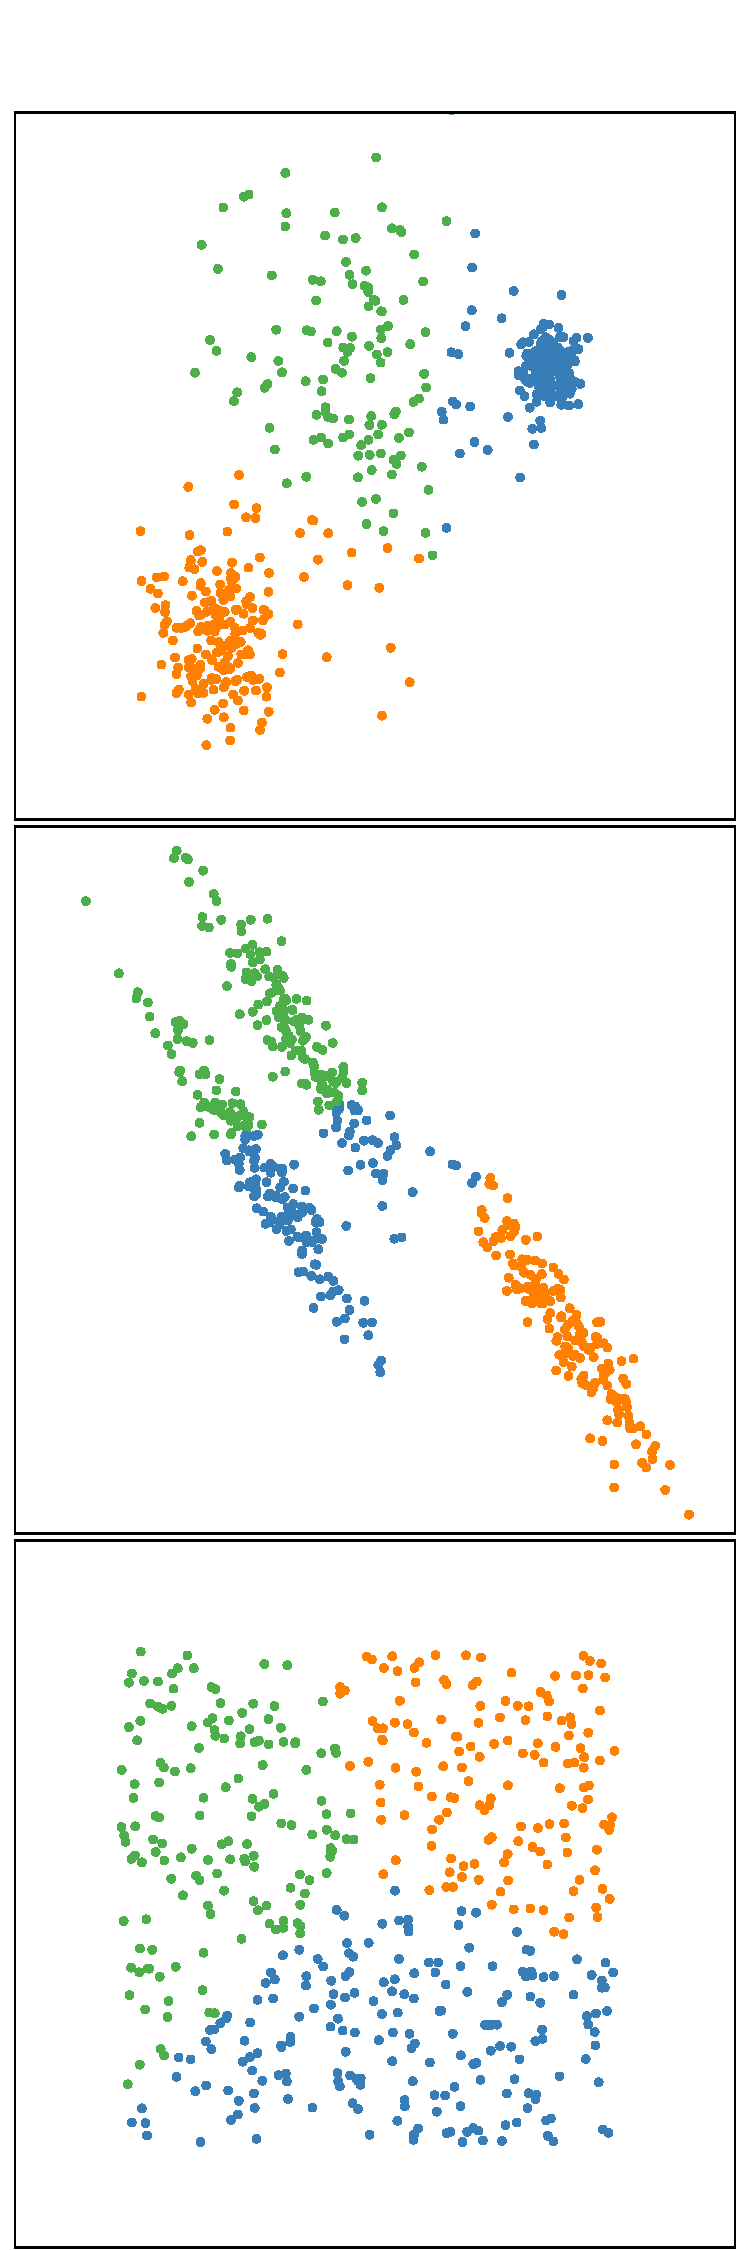
\includegraphics[height=15cm, angle=90]{Bilder/models/minibkmeans.pdf}
		\caption{How MiniBatchKmeans recognizes Clusters \cite{sklearn}}
		\label{fig:kmeans-viz}
		\end{figure}
	
		The k-Means algorithm performs reasonably well in identifying clusters in data such as in figure \ref{fig:kmeans-viz}. The left example seems unspectacular, but in the center example, it becomes obvious that k-Means is prone to overfit on noisy data. This can be partially blamed on the focus on centers, and not density. The focus on centers is also obvious in the rightmost example. While the data is quite evenly distributed over the area, the algorithm still groups the data. 
		
		Implementations such as \ac{sklearn}'s \lstinline|MiniBatchKMeans| \cite{sklearn} speed up the computation time by processing subsets of the data in a parallel way. While only achieving almost perfect results \cite{sculleyWebscaleKmeansClustering2010}, the batched k-Means algorithm is of special appeal when handling large data sets.
		
		This algorithm has the advantage of high performance, and performs well on large data sets. Unfortunately, the quality of the results depend highly on choosing the correct parameters. Also, k-Means is not robust against outliers, and results are not reproducible since the first cluster centers are chosen randomly \cite[c.6.2]{40algorithms}.
		
		\subparagraph{\acl{DBSCAN}}
		The \ac{DBSCAN} clustering algorithm was developed to solve the problem of needing domain knowledge while tuning cluster models \cite{DBSCAN}. The algorithm uses an intuitive approach for identifying which points belong into a cluster, and which are outliers.

		For two points to be considered neighboring (density-reachable, \cite{DBSCAN}), they have to be within a certain distance to each other: \lstinline|eps|. Neighboring points are categorized into one cluster, expanding the reach of this cluster over all values within the distance \lstinline|eps|.
		But, there is a limitation to the points being able to expand a cluster. If the cluster were to expand without limitations apart from a maximum distance, the clusters would be able to "spread" from one cluster to another if connected by one data point.
		To prevent this, only center points can expand the cluster. A center point has a minimum number of neighboring points (\lstinline|min_samples|). This helps to create dense clusters and prevents the undesirable spreading.
		
		 \begin{figure}[!h]
			\centering
			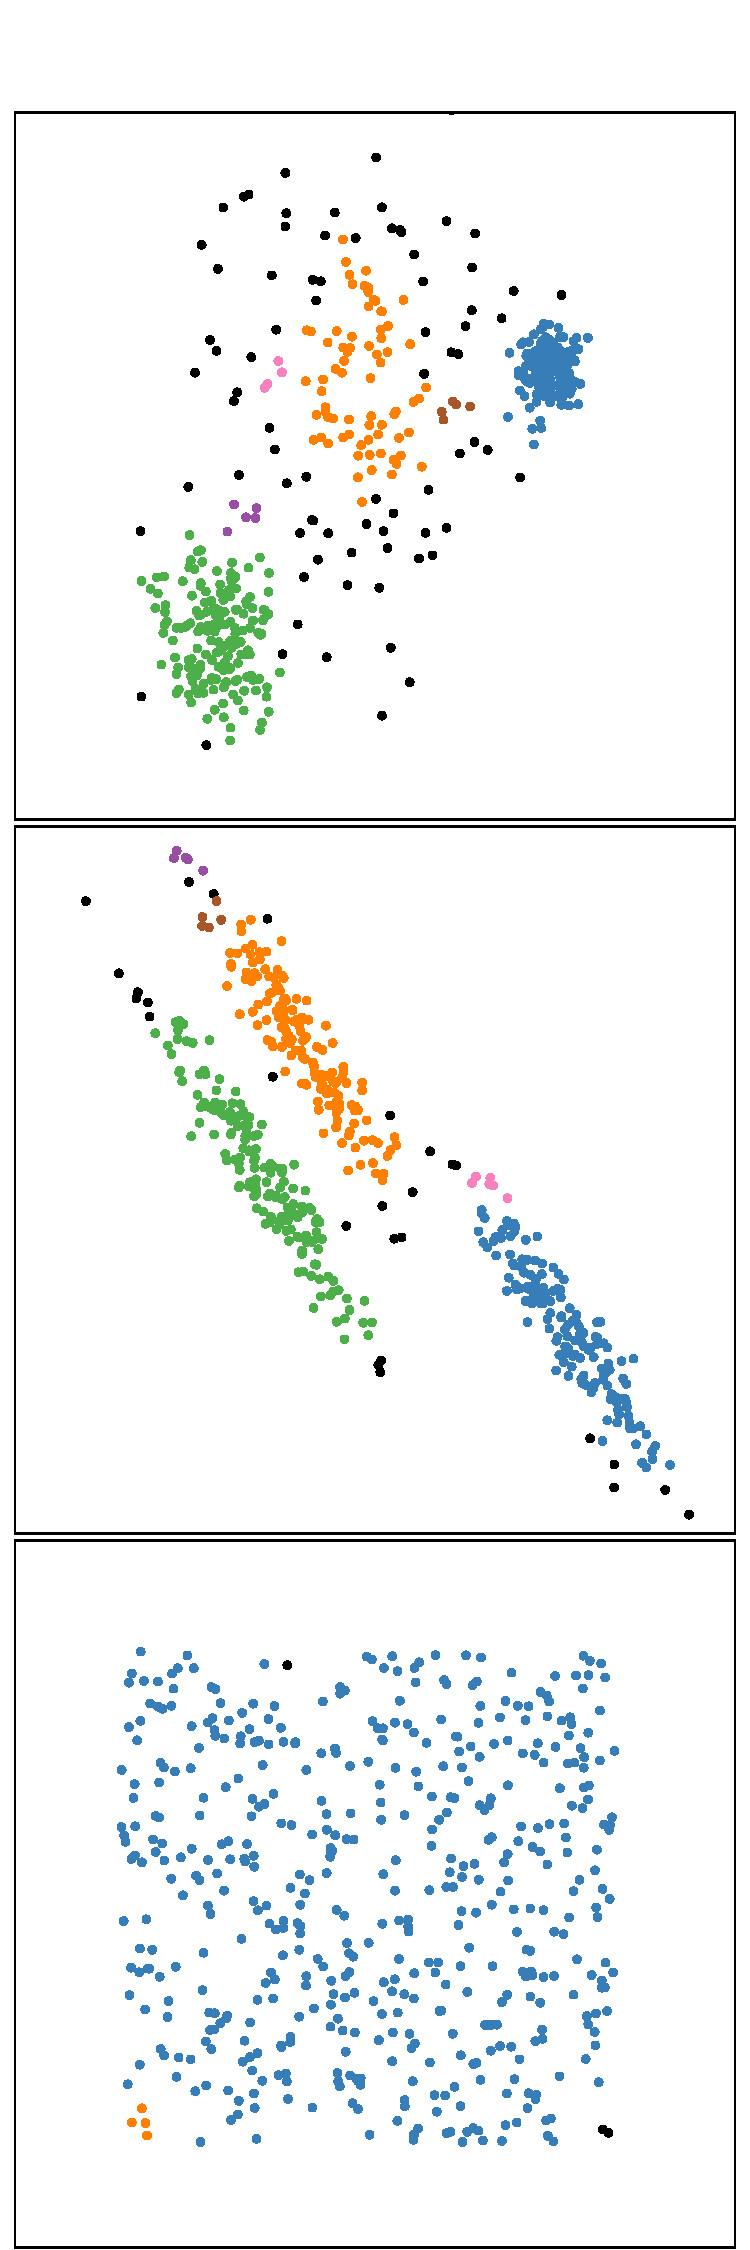
\includegraphics[height=15cm, angle=90]{Bilder/models/dbscan.pdf}
			\caption{How DBSCAN recognized Clusters and Outliers \cite{sklearn}}
			\label{fig:dbscan-viz}
		\end{figure}
	
		Figure \ref{fig:dbscan-viz} illustrates how \ac{DBSCAN} does not fall prey to outliers, as k-Means does. A broad distribution of data points in the left example is very intuitively grouped into clusters and outliers. Especially the center picture showcases the ability of DBSCAN to recognize clusters by their density. The even spread of data in the third example is also correctly identfied as one large cluster, even though a small part of the data was not within \lstinline|eps| range.
		
		

		
\subsection{Topic Model}

\subsection{Dimensionality Reduction}

\section{Theoretical Implementation}
\begin{enumerate}
	\item Determining composition of dataset with KNeighbors Algorithm.
	\item Preselect documents with \ac{DBSCAN} and cosine distance.
	\item Determine the number of clusters with the Elbow Method.
	\item Train a KMeans Model with cosine distance.
	\item Visualize cluster formation.
	\item Generate Topics per cluster with \ac{LDA}.
\end{enumerate}



\section{Practical Implementation}

\subsection{Determining composition of dataset with KNeighbors Algorithm}


Both density-based and distance-based clustering algorithms work with distances between objects. Before any clustering is applied, an overview over the distances should be established \cite{maklinDBSCANPythonExample2022a}. This allows to make meaningful decisions while hyperparameter-tuning.

 \begin{figure}[!h]
	\centering
	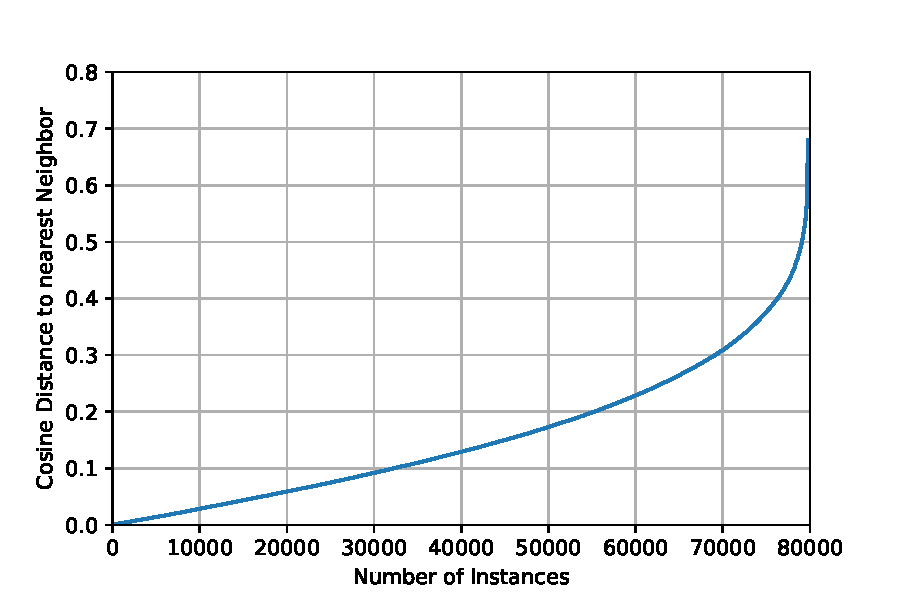
\includegraphics[height=8cm]{Bilder/models/kneighbors.pdf}
	\caption{Each Instance's Distance to the nearest neighboring Point}
	\label{fig:dbscan-plot}
\end{figure}

This can be done with the algorithm \lstinline|sklearn.neighbors.NearestNeighbors|, which takes the input of a dataset with arbitrary dimensions. Using a specified distance metric, the algorithm outputs the distance of each data point to its nearest neighbor in the data set. The distance metric used is the cosine distance.
The distance search shows that almost all points are within a maximum distance of 0.4 to the next neighbor. All other points are outliers and will be filtered out with \ac{DBSCAN}.



\subsection{Preselect documents with \ac{DBSCAN} and cosine distance}
The \ac{DBSCAN} algorithm outputs, apart from clusters, outlier data points which do not belong into any cluster. With this algorithm, outliers in the data are detected to prevent the main clustering algorithm (KMeans) from overfitting. 
The clustering algorithm has the parameters \lstinline|eps| and \lstinline|metric| which tune the model.

The (distance) \lstinline|metric| is of course cosine. The \lstinline|eps| stands for the maximal distance between two points to be considered a neighbor \cite{SklearnClusterDBSCAN}. As established before, the outliers are those points which are more than 0.4 units separated from the next data point. Therefore, \lstinline|eps| is set to 0.4. 

The \ac{DBSCAN} model identified the outlier data (\ref{fig:dbscan-outliers}), amounting to about 3\% of the data points. These data points are not included into clustering by k-Means.

\subsection{Determine the number of clusters with the Elbow Method}
The KMeans algorithm is parameterized with the number of clusters (\lstinline|n_clusters|). Since the algorithm itself is not able to determine the cluster count, this number has to be approximated.
\cite{kodinariyaReviewDeterminingCluster2013} suggest several applicable methods, among them are rule of thumb, and the elbow method with a silhouette score.
A good point for starting with choosing \lstinline|k| is the rule of thumb $k \approx \sqrt{\frac{n}{2}}$ with n being the number of instances in the dataset. Other literature also names the approximation of $k \approx log(n)$, but \cite{maierOptimalConstructionKnearest2009} showcase how $k$ should be chosen in the order of $n$. 

\begin{table}[!h]
	\centering
	
	\begin{tabular}{l|ll}
		\toprule
		heuristic for best k                         & k &  \\
		\midrule
		$k \approx \sqrt{\frac{n}{2}}$ &  199 &  \\
		$k \approx log(n)$             & 12   &  \\
		$k \approx n$                  &  e.g. 10 000, 20 000& 
	\end{tabular}
\caption{Three possible estimates for the optimal $k$}
\label{table:heuristic-k}
\end{table}

With the elbow method, the silhouette score of clustering results for different values of \lstinline|k| are visualized. 

The silhouette score is a measure of how similar intra-cluster points are and at the same time how dissimilar inter-cluster points are. A silhouette score of 1, being the highest value, is the most desirable.

The silhouette score $s$ of each data point $i$ can be calculated with the following formula \cite{kodinariyaReviewDeterminingCluster2013}:
\[ s(i) = \frac{b(i) - a(i)}{\max\{a(i),b(i)\}} \]

The measure $a$ denotes the mean distance to other points in the same cluster as $i$. This is interpreted as the inter-cluster dissimilarity, the higher $a(i)$, the more $i$ doesn't belong into the cluster.

The measure $b$ stands for the mean distance between $i$ and the points in the nearest other cluster. To identify the nearest other cluster to the point $i$, all mean distances to points of each cluster are calculated. The cluster with the smallest mean distance between all its points and $i$ is the neighboring cluster. The measure $b$ is interpreted as the similarity of $i$ to other clusters.

Being calculated for every point, this measure always falls in the interval $[-1;1]$. For $S = 1$, the relationship of $a(i)$ and $b(i)$ has to be $a(i) \ll b(i)$ so that the denominator and divisor each tend to $b(i)$ resulting in $S = 1$. This would mean that the point $i$ would have to be very far away from points in other clusters and very near to its own cluster. The value $S = 1$ is therefore the most desirable.

For $S = 1$, the relationship of $a(i)$ and $b(i)$ has to be $a(i) \gg b(i)$ so that the denominator and divisor each tend to $-a(i)$ respective $a(i)$ resulting in $S = -1$. In distance terms this means that the point $i$ is very far away from its own cluster points and very close to points in the next nearest cluster.

Therefore, the task of the elbow method using the silhouette coefficient is to maximize $S$ while preventing overfitting.

The above mentioned estimates (\ref{table:heuristic-k}) are a starting point for choosing values for k during the calculation of silhouette coefficients.


\subsection{Train a KMeans Model}

\subsection{Visualize cluster formation}
\subsection{Generate Topics per cluster with \ac{LDA}}



		